\begin{frame}[c]
  \frametitle{Gene regulations}

\begin{center}
    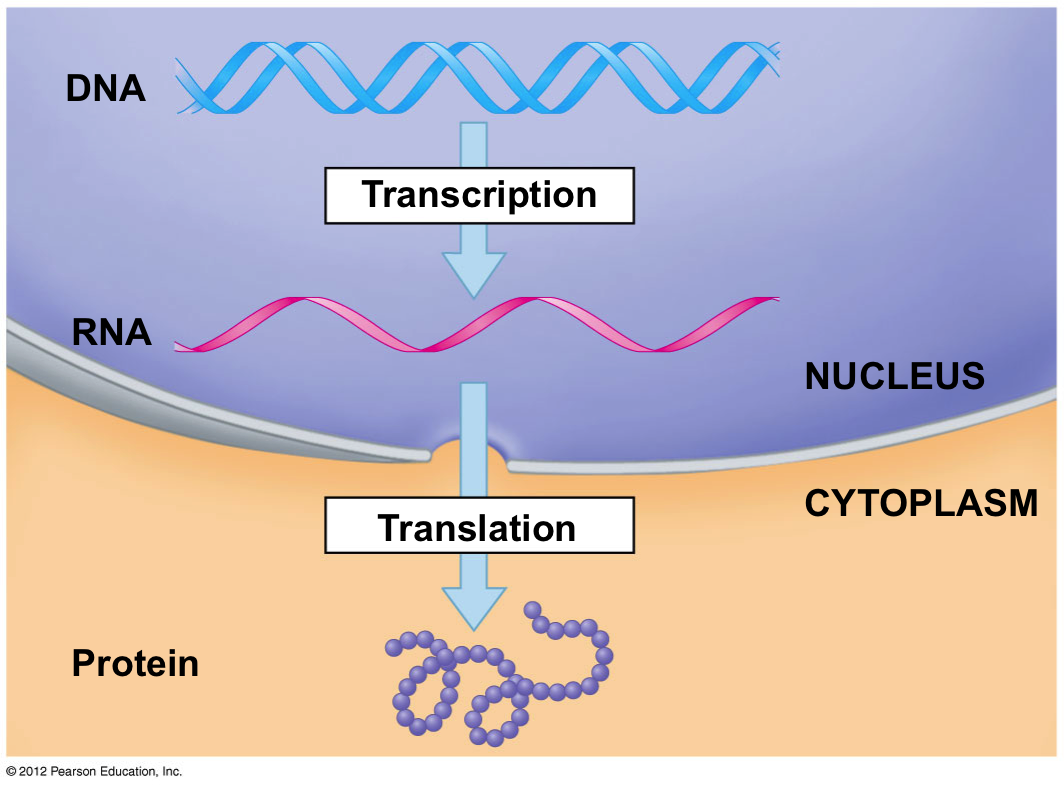
\includegraphics[width=.4\textwidth]{figs/protein.png}
    \uncover<2>{
      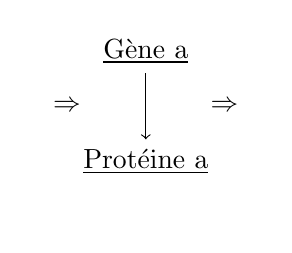
\begin{tikzpicture}
        \path[use as bounding box] (-3, 1) rectangle (0, -1.5);
        \node at (-1.5,.7) (ga) {\underline{Gène a}};
        \node at (-1.5,-0.7) (pa) {\underline{Protéine a}};
        \node[draw=none] at (-2.5,0) {$\Rightarrow$};
        \path[draw,->] (ga) -- (pa);
        \node[draw=none] at (-0.5,0) {$\Rightarrow$};
      \end{tikzpicture}}
    \uncover<2>{
      \scalebox{2}{
      \begin{tikzpicture}[adn]
        \path[use as bounding box] (-.3, .5) rectangle (0.5, -.7);
        \node (a) {a};
      \end{tikzpicture}}
    }
\end{center}

\end{frame}